\documentclass[10pt]{article}

\usepackage{amsmath}
\usepackage{amsfonts}
\usepackage{amssymb}
\usepackage{amsthm}
\usepackage{microtype}
\usepackage{asymptote}
\usepackage{graphicx}
\usepackage[affil-it]{authblk}
\setlength\parindent{10pt}

\begin{document}
\author{Jacob Bruner}
\title{MYP 1.3 ACD \\ Temperature of a Cup of Hot Water Over Time}
\date{November 23, 2020}
\affil{Advanced Algebra and Calculus I Honors \\ The Dwight School}
\maketitle

\begin{asydef}
import graph;
import math;
\end{asydef}



\section{Overview}

A cup of water was filled from the hot water spigot on the water cooler in North Campus. That water was left, uncovered, in a room. A thermometer was used to continuously monitor the water's temperature.

Temperatures were recorded at various times in the table below:

\begin{figure}[h]

\begin{center}
\begin{tabular}{|c c| c|}
	
	\hline
		Time (in HH:MM)& $\Delta t$  (in min) & $u$ (in $^\circ$F)
	\\ \hline \hline
		10:42 & 0 & 147.6\\
		10:47 & 5 & 136.0\\
		10:50 & 8 & 133.2\\
		10:58 & 16 & 123.0\\
		11:06 & 24 & 114.6\\
		11:07 & 25 & 113.2
	\\ \hline
\end{tabular}
\caption{Temperatures Recorded at Various Times}
\end{center}

\end{figure}
In addition, the constant ambient temperature of the room was 77.1 $^\circ$F


\section{Spatially Independent Evaluation}
\subsection{Derivation}
\textit{\textbf{Newton's Law of Cooling} states that the the rate of heat loss of a body is directly proportional to the difference in temperature between the body and its surroundings,} under the primary assumption that the temperature of the surroundings is constant, in that the surroundings are \textit{much more vast} than the body,  so its change in temperature will be negligibly small. This can be written in the form of a differential proportion:
	\begin{equation} \label{1}
	\frac{\partial{u}}{\partial{t}} \propto u-u_{a}
	\end{equation}
Where $u$ is the temperature of the body and $u_{a}$ is the temperature of the ambient environment. \\
Under the simplifying assumption that a proportionality constant (in this case a heat transfer coefficient) is independent of the difference in temperature and the location with respect to the environment,
%     mention in error section note convection and conduction, note change in heat velocity (both in both spatial and nonspatial), note change in heat throughout body not uniform 
(\ref{1}) will be satisfied by a negative real number (negative because, logically, the temperature of the body approaches the ambient temperature), denoted with $-k$:
	\begin{equation}
	\forall \dot{u},\ \forall (u-u_a),\ \exists k>0\ |\ \dot{u} = -k \Big( u-u_{a} \Big)
	\end{equation}
From here, this First-Order Linear Differential Equation is easily solvable with variable separation and integration on both sides:
	\begin{align}
	\frac{du}{dt} &= -k \Big( u-u_{a} \Big) \notag \\
	\frac{1}{( u-u_{a} )}\ du &= -k \ dt \notag \\ 
	\int \frac{1}{( u-u_{a} )}\ du &= \int -k\ dt \label{eq:3} \\
	\ln \Big| u-u_{a} \Big| &= -kt + C_1 \label{eq:4}
	\end{align}
Solving \eqref{eq:4} for temperature at time $t$ by exponentiation by e:
	\begin{align*}
	\ln \Big| u-u_{a} \Big| &= -kt + C_1 \notag \\
	\Big| u-u_{a} \Big| &= e^{-kt + C_1} \notag \\
	\Big| u-u_{a} \Big| &= e^{-kt} \times e^{C_1}
	\end{align*}
Here, $e^{C_1}$ is another constant resulting from exponentiation by e, and thus, will be represented by $C$. 
	\begin{equation}
	\Big| u-u_{a} \Big| = Ce^{-kt}  \label{eq:5}
	\end{equation}
	
This absolute value creates two instances of  the solution. In a situation where the body is hotter than the environment (as in $u-u_{a}$ is positive), a solution can be obtained like so:
	\begin{align*}
	u-u_{a} &= Ce^{-kt}\\
	u &= Ce^{-kt}+u_{a}
	\end{align*}
So when $\left \lbrace  u > u_a \right \rbrace $, this function satisfies the initial statement:
	\begin{equation}
	\label{eq:6}
	u(t) = Ce^{-kt}+u_{a}
	\end{equation} \\
Similarly, in a situation where the body is less hot than the environment ($u-u_{a}$ is negative), a solution can be obtained like so:
	\begin{align*}
	\Big| u-u_{a} \Big| &= Ce^{-kt}\\
	-(u- u_{a}) &= Ce^{-kt}\\
	-u+u_{a} &= Ce^{-kt}\\
	-u &= Ce^{-kt}-u_{a}\\
	u &=u_{a}-Ce^{-kt}
	\end{align*}
So when $\left \lbrace  u < u_a \right \rbrace $, this function satisfies the initial statement:
	\begin{equation}
	u(t) =u_{a}-Ce^{-kt}\label{eq:7}
	\end{equation}
\subsection{Application}

\subsubsection{Solution From Initial Conditions}

An important piece of information from \eqref{eq:7}, the $C$ coefficient, is required to solve this equation for $-k$. Because there are two unknown constants, the ability to find solutions to this differential equation is limited. However luckily, two small points were missed while integrating. The bounds of the integrals in \eqref{eq:3}! In this application, it should look like the following: (because $\lbrace u > u_a \rbrace$ and $\lbrace t \geqslant 0 \rbrace$)
	\begin{align}
	\int_{\Delta u_0}^{\Delta u} \frac{1}{\Delta u}\ du &= \int_{0}^{t} -k\ dt \label{eq:8}
	\end{align}
Where $\Delta u$ is $u-u_{a}$, and $\Delta u_0$ is this temperature difference at the start.\\Therefore, solving \eqref{eq:8} for $u(t)$:
	\begin{align}
	\ln  \Delta u \Big|_{\Delta u_0}^{\Delta u} &= -kt  \notag \\
	\ln (\Delta u) - \ln (\Delta u_0) &= -kt \notag \\
	\ln \bigg( \frac{  \Delta u  }{  \Delta u_0  } \bigg) &= -kt \notag \\
	\bigg( \frac{  \Delta u  }{  \Delta u_0  } \bigg) &= e^{-kt} \notag \\
	\Delta u &= \Delta u_0 (e^{-kt}) \label{eq:9}
	\end{align}
And re-substituting $u-u_{a}$ for $\Delta u$ in \eqref{eq:9}, we get the general solution for these circumstances:
	\begin{align}
	u-u_{a} &= u-u_{a} (e^{-kt})\notag\\
	u(t) &= u_{a}+(u_0-u_{a}) e^{-kt} \label{eq:10}
	\end{align}


\subsubsection{Approximating A Function Using Room Temperature and Water Temperature Measurements}
From \eqref{eq:10}, the constant $-k$ can be approximately solved for using the measured values, specifically: the initial temperature of the  body $(u_0)$, the ambient temperature $(u_a)$, and any pair of time and temperature $(t,\ u(t))$. Solving for $-k$, and showing work as required:
	\begin{proof}
	Using $u_0 = 147.6$, $u_a = 77.1$, and the pair $t=16,\ u(16) = 123$; solve k from 				\eqref{eq:10} over the real numbers.
	\begin{align*}
		u(t) &= u_{a}+(u_0-u_{a}) e^{-kt} && \text{(given)} \\
		123 &= 77.1+(147.6-77.1) e^{-k(16)} && \text{(substitution)}\\
		45.9 &= 70.5e^{-16k} && \text{(def $\pm$)} \\
		\frac{45.9}{70.5} &= e^{-16k}  && \text{(def $\div$)}  \\
		\ln \bigg( \frac{45.9}{70.5} \bigg)&= -16k && \text{(def $\div$)} \\
		k &= -\frac{\ln \big( \frac{45.9}{70.5} \big)}{16}&& \text{(def log)} \\
		k &\approx 0.026822 && \text{(def calculator)} 
  		%
		%                 s &= s  && \text{(  )} 
	\end{align*} 
	\end{proof}
Then substituting this solved value of $k$ and the values of the ambient and initial temperatures into \eqref{eq:10}, a function for temperature $u$ (in $^\circ$Fahrenheit) at a given time $t$ (in minutes) is determined:
	\begin{align}
	u(t) &= 77.1+(147.6-77.1) e^{-(0.026822)t} \notag \\
	u(t) &= 77.1+ 70.5 e^{-0.026822t} \label{eq:11}
	\end{align}
Now, this function can be used to make predictions about the cup of water cooling.

\subsubsection{Making Predictions}
Although the value of $k$ was only solved for using one data point, the function can be used to make predictions to a reasonable degree of accuracy.

 One temperature I am particularly curious about is 130$^\circ$F; it is my favorite temperature for drinking tea! I tested this on my own by brewing a cup of green tea and using a thermometer when I felt that it was the best temperature for drinking. The result of this mini-experiment, was that I enjoy tea around 130$^\circ$F.\newpage 
Now, \eqref{eq:11} can be used to predict how long after the heating of a cup of water to $\sim$147$^\circ$F in a 77.1$^\circ$F room would cool to 130$^\circ$F:
	\begin{align*}
	130 &= 77.1+ 70.5 e^{-0.026822t}\\
	52.9 &= 70.5 e^{-0.026822t}\\
	\frac{52.9}{70.5} &= e^{-0.026822t}\\
	\ln \bigg( \frac{52.9}{70.5} \bigg) &= -0.026822t \\
	t &=   - \frac{\ln \big( \frac{52.9}{70.5} \big)    }{0.026822}  \\
	t &\approx     10.708 \min \\
	\text{or... } t &\approx     10 \min 42 \sec 
	\end{align*}
Similarly, if one wanted to predict what temperature that cup of water would be at 30 minutes after heating it, it could be done like so using \eqref{eq:11}:
	\begin{align*}
	u(30) &= 77.1+ 70.5 e^{-0.026822(30)}\\
	&= 77.1+ 70.5 e^{-0.80466}\\
	&\approx 77.1+ 70.5(0.44724)\\
	&\approx 77.1+ 31.5304\\
	u &\approx 108.6 ^\circ \text{F}
	\end{align*}
\newpage


\subsubsection{Validity of Predictions and Equation}

Although this method of finding an equation is not the most rigorous--especially in that it only factors in one data-point--it is able to provide a result that is both reasonable, and within a margin of error such that it is useful in the real world. 

One useful way of visualizing the accuracy of an equation from one data point is to compare it to the other measurements taken. This is accomplished by graphing \eqref{eq:11} with temperature on the y-axis and time on the x-axis, then plotting the various measurements as points over it. This graph is featured below, including the room temperature as a line to show the asymptotic behaviour of the function:
	\begin{figure}[h!]
	\begin{center}
		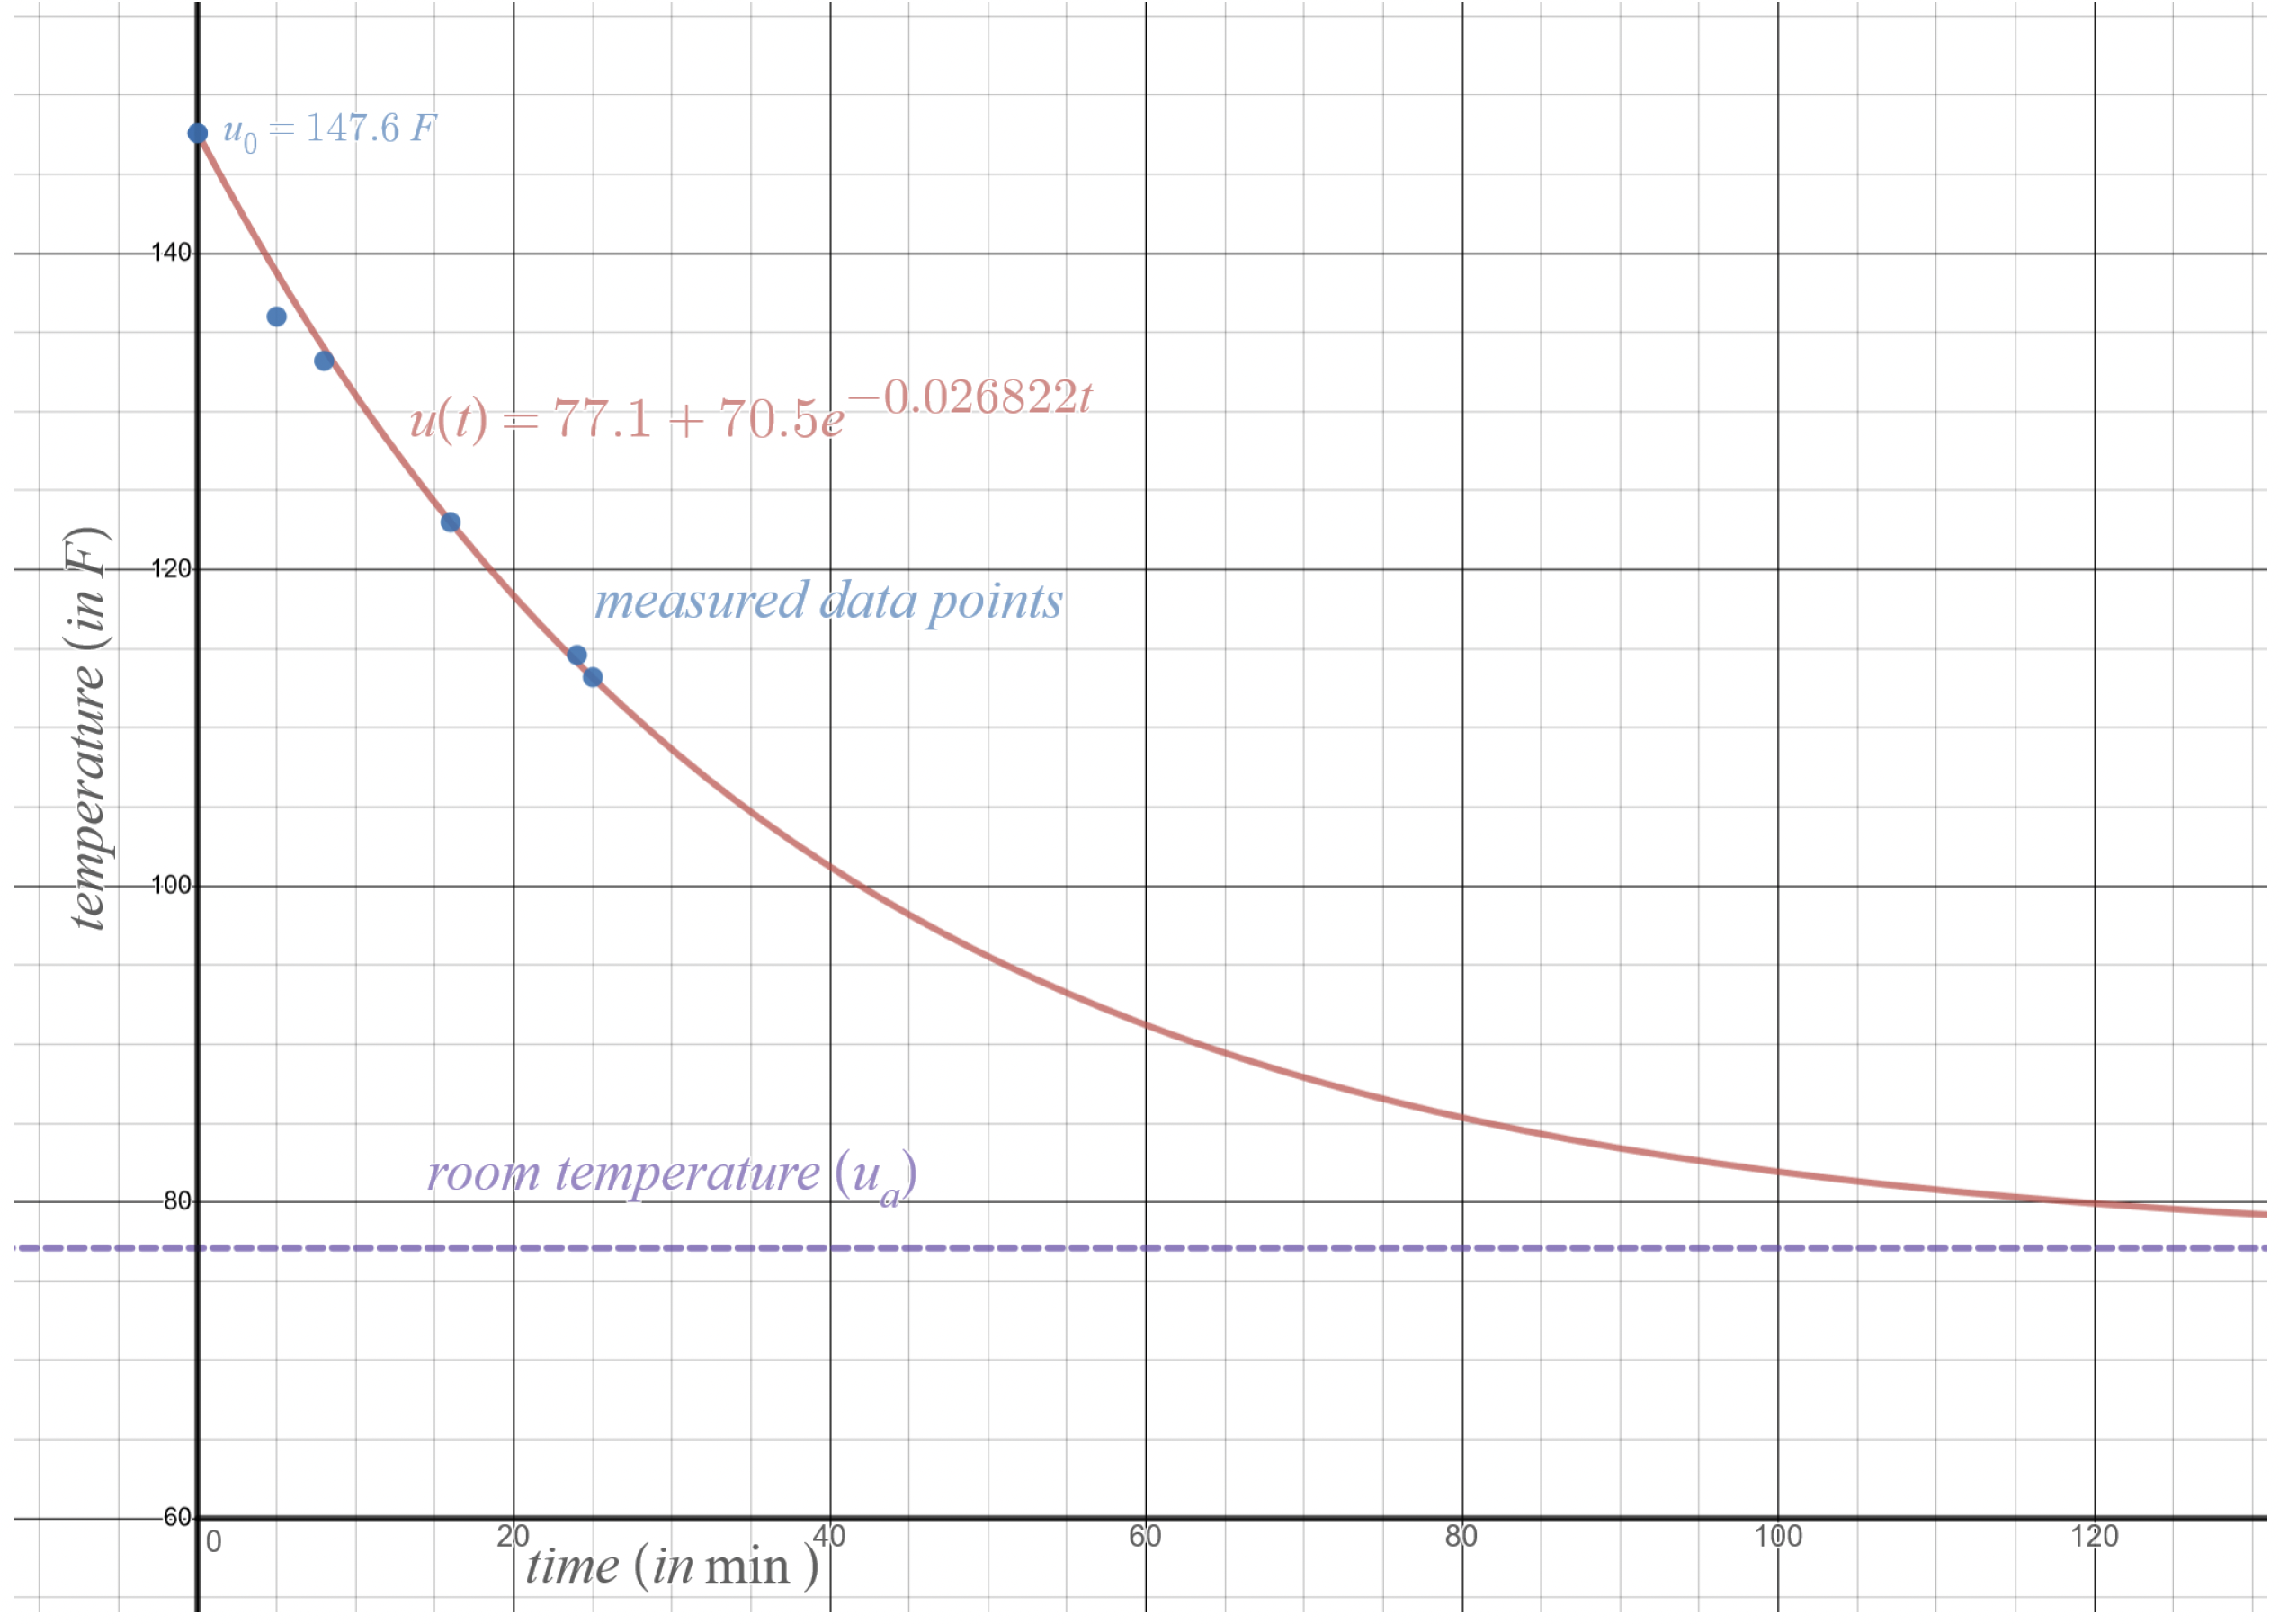
\includegraphics[scale=.3]{graphheat}
		\caption{Temperature $u$ over Time $t$}
		\label{fig:2}
	\end{center}
	\end{figure} \\
From [\ref{fig:2}] it is clear that the function (in red) fits the data-points (in blue) to a reasonable degree of accuracy. The first few temperature measurements fall a little under the predictions, however the points after fit the model well. Despite this, the equation is based off one data-point, and therefore wholly reflects any error in measurement or time that point may have had. Ideally, multiple data-points would be used because the error would even out with more information. Data should have also been collected over a longer period of time, so the decaying behavior of the temperature could be more clearly demonstrated. The measurements do not conclusively demonstrate an exponential decay; the points shown could possibly have been connected in a line. Either way, for most intensive purposes, I believe this equation to be an--for the most part--accurate model of how the temperature of the water decays over time, despite limitations.

\subsection{Limitations}
This exponential solution makes a lot of assumptions about the nature of the experiment. One of the primary assumption Newton's Law of Cooling assumes is that the heat transfer mechanism stays the same. With water this is false. As water is cooled down, the rate at which it absorbs heat increases. This law realistically only applies well to convective heat transfer. When a cup of water dissipates heat, it is preforming conductive cooling from the water to the air, and because water and air are different liquids, the mechanism of heat transfer changes as the temperatures change relative to each other.

Furthermore, this law generalizes a body to be a 'lumped capacitance object' meaning that the temperature is uniform throughout. Although this is a somewhat minor assumption, it is still critical to recognize that the water would cool faster closer to the place where it makes contact with the air. The more nuanced and correct solution to this example would be the general diffusion and heat equation. Where similarly it postulates that the rate of change in temperature is proportional to the difference in temperature between it and its surroundings, except that it does this for arbitrarily small changes in temperature over a distance. This is accomplished by measuring the divergence of the gradient at all points in space. Which--intuitively--measures if the rate at which temperature changes ($\nabla u$) at points around a position has a tendency to move toward or away from that point ($\nabla \cdot (\nabla u)$). At a high level it compares the change of temperature at values around a point and outputs whether it will increase or decrease compared to the average of its neighbors. Notated with the laplacian $\nabla^2$, this makes the simple ODE from Newton's Law of Cooling into the quintessential example of a difficult partial differential equation: $\dot{u}=\nabla^2 u$. Or written in a way that does its difficulty more justice (in $\Re^3$, Cartesian coordinates without a proportionality constant):
\begin{align*}
	\dot{u} &= u_{xx} + u_{yy} + u_{zz}\\
	&\textit{or}\\
	\dfrac{\partial u}{\partial t} &= \dfrac{\partial^2 u}{\partial x^2} + \dfrac{\partial^2 u}{\partial y^2} + \dfrac{\partial^2 u}{\partial z^2}
\end{align*}
 The solution to this changes from an equation a calc 1 student could solve, to the type of equation that an entire college course--multivariate calculus--is dedicated to. Despite this, it isn't a shockingly unreasonable assumption that the temperature at a point is the same as its neighbors in a homogeneous body, because in this case especially, temperature only would significantly vary with time, not position from the contact with air.
 
It is worth mentioning that despite limitations in mathematical methods of approximation, real world error would arguably have more direct influence on the validity of the results or predictions. For example, the measurement in this experiment was done with time precision up to a minute. The temperature change between the water at 1 minute 0 seconds and 1 minute 59 seconds is significant enough that it may have affected the accuracy of the data. Another variable not controlled for is the ambient temperature of the room. The room may have heated up or cooled down contributing to the temperature of the water. Likewise the water was not instantly heated to its initial temperature, so its more than likely that the initial temperature used is not actually the initial temperature.

Overall, it is a difficult task to eliminate error or difficulty in performing an experiment. In this experiment, there were a number of factors and generalizations that may have contributed to error, however I think that (as long as taken with skepticism and doubt) the solutions provided in this mathematical and experimental setup are to a great extent valid models of the real world for most purposes.


\end{document}
